% Тут используется класс, установленный на сервере Papeeria. На случай, если
% текст понадобится редактировать где-то в другом месте, рядом лежит файл matmex-diploma-custom.cls
% который в момент своего создания был идентичен классу, установленному на сервере.
% Для того, чтобы им воспользоваться, замените matmex-diploma на matmex-diploma-custom
% Если вы работаете исключительно в Papeeria то мы настоятельно рекомендуем пользоваться
% классом matmex-diploma, поскольку он будет автоматически обновляться по мере внесения корректив
%

% По умолчанию используется шрифт 14 размера. Если нужен 12-й шрифт, уберите опцию [14pt]
%\documentclass[14pt]{matmex-diploma}
\documentclass[14pt]{matmex-diploma-custom}
\usepackage{fontspec}
\usepackage{polyglossia}
\usepackage{amsmath}
\usepackage{amsfonts}
\usepackage{amssymb}

% пакеты из презентации
\usepackage{algpseudocode}
\usepackage{algorithm}
\usepackage{algorithmicx}
\usepackage{pdfpages}

\usepackage{subcaption}
\usepackage{geometry}
\usepackage{amsfonts,latexsym}
\usepackage{amsthm}
\usepackage{amssymb}
\usepackage[utf8]{inputenc} % Кодировка
\usepackage{mathtools}
\usepackage{hyperref}
\usepackage{tikz}
\usepackage{dsfont}
\usepackage{multicol}
\usetikzlibrary{fit,calc,automata,positioning}

\theoremstyle{definition}
\newtheorem{rudefinition}{Определение}[section]
\newtheorem{example}{Пример}[section]
\newtheorem{theorem}{Теорема}[section]
\newtheorem{proposition}[theorem]{Proposition}
\newtheorem{lemma}[theorem]{Лемма}
\newtheorem{corollary}[theorem]{Corollary}
\newtheorem{conjecture}[theorem]{Conjecture}
\newtheorem{note}[theorem]{Утверждение}

\begin{document}
% Год, город, название университета и факультета предопределены,
% но можно и поменять.
% Если англоязычная титульная страница не нужна, то ее можно просто удалить.
\filltitle{ru}{
    chair              = {Программная инженерия},
    title              = {Улучшение производительности алгоритма поиска путей с контекстно-свободными ограничениями для графовой базы данных Neo4j},
    % Здесь указывается тип работы. Возможные значения:
    %   coursework - Курсовая работа
    %   diploma - Диплом специалиста
    %   master - Диплом магистра
    %   bachelor - Диплом бакалавра
    type               = {coursework},
    position           = {студента},
    group              = 371,
    author             = {Погожельская Влада Владимировна},
    supervisorPosition = {к.\,ф.-м.\,н., доцент кафедры информатики},
    supervisor         = {Григорьев С.\,В.},
%   university         = {Санкт-Петербургский Государственный Университет},
%   faculty            = {Математико-механический факультет},
%   city               = {Санкт-Петербург},
%   year               = {2020}
}
\maketitle
\tableofcontents
% У введения нет номера главы
\section*{Введение}
Графовая модель данных широко используется во многих областях \cite{robinson2015graph}, таких как, например, графовые базы данных \cite{10.1145/2463664.2465216}, биоинформатика \cite{rna}, статический анализ кода \cite{10.1145/2499370.2462159} и т.д. Основное преимущество данной модели над реляционной моделью данных заключается в том, что получение информации об отношении между объектами в ней выполняется очень быстро, поскольку взаимосвязи между узлами не вычисляются во время выполнения запроса, а хранятся в самой модели. Одной из самых распространенных задач, связанной с анализом данных, представляемых с помощью графов, является поиск путей. В графовых базах данных для их анализа используются запросы, естественным способом задания которых является наложение ограничений на пути между вершинами.

Одним из подходов для выражения таких запросов является определение формальных грамматик над алфавитом меток ребер. Путь принадлежит языку, задаваемому формальной грамматикой, если ему принадлежит слово, получаемое конкатенацией меток ребер данного пути \cite{arcbool}.  Наиболее часто при таком подходе в качестве грамматик берутся регулярные. Так, например, в одной из наиболее распространенных графовых баз данных Neo4j в качестве языка запросов используется декларативный язык Cypher \cite{cypher}, поддерживающий ограничения на пути, заданные в терминах регулярных языков. Причем стоит отметить, что регулярные ограничения поддерживаются лишь частично и на текущий момент язык запросов довольно ограничен. Одним из способов расширить выразительность запросов является переход к ограничениям в терминах контекстно-свободных языков. Они строго расширяют выразительность запросов по сравнению с регулярными языками и тем самым позволяют решать более широкий класс задач. Одной из таких задач является запрос поиска всех потомков одного поколения (same-generation query). Она выразима в терминах контекстно-свободных языков, но не в терминах регулярных выражений \cite{10.1007/978-3-319-91662-0_17}.

Несмотря на то, что проблема поиска путей, удовлетворяющих ограничениям в терминах формальной грамматики, довольно хорошо изучена и существуют множество различных алгоритмов для ее решения \cite{10.1145/3210259.3210264, zhang2016contextfree, hellings2016querying, medeiros2020algorithm}, все еще существует ряд проблем, связанных с их применимостью в анализе реальных данных \cite{10.1145/3335783.3335791}. Одной из наиболее остро стоящих проблем является низкая производительность существующих алгоритмов, поэтому актуальной задачей является разработка и реализация новых алгоритмов, решающих данную проблему.

Одной из недавних разработок является адаптация классического алгоритма синтаксического анализа Generlized LL для выполнения контекстно-свободных запросов на графах\footnote{GitHub репозиторий реализации обобщенного GLL алгоритма: \url{https://github.com/YaccConstructor/iguana},  дата обращения: 15.12.2020}.
Важно отметить, что полученный алгоритм поддерживает весь класс контекстно-свободных языков. Тем не менее при проведении экспериментального исследования полученного алгоритма при выполнении ряда запросов было выявлено резкое снижение производительности. Модифицированный GLL, так же как и оригинальный алгоритм, возвращает информацию не только о достижимостях между вершинами, но и информацию для построения самих путей. Для этого используется специальная структура данных --- сжатое представление леса разбора (SPPF).
Однако, данная структура потребляет значительное количество ресурсов и, как следствие, замедляет работу всего алгоритма. На практике же, ограничения на процессорные ресурсы являются весьма существенными, при этом восстановление самих путей не всегда требуется --- достаточно получить лишь информацию о самом их существовании. Таким образом, была выдвинута гипотеза о том, что добавление возможности отключения построения SPPF даст ощутимый прирост в скорости выполнения запросов на реальных данных. Данная работа направлена на улучшение производительности разработанного алгоритма и, в частности, на проверку этой гипотезы. 


\section{Постановка задачи}
Целью данной работы является улучшение производительности алгоритма поиска путей с контекстно-свободными ограничениями для графовой базы данных Neo4j.

Для достижения поставленной цели были выделены перечисленные ниже задачи.
\begin{itemize}
    \item Проведение анализа кода и его рефакторинг с целью выявления и устранения проблем производительности текущей реализации GLL алгоритма.
    \item Добавление возможности отключения построения SPPF и возвращения информации лишь о достижимостях в графе.
    \item Проведение экспериментального исследования на реальных данных и сравнение полученного решения с уже существующим.
\end{itemize}

\section {Обзор}
В данный раздел включены основные определения с дальнейшим описанием как теоретической части алгоритма, так и его реализации.
\subsection{Понятия из теории формальных языков}
Введем базовые определения из теории формальных языков, которые будут использоваться в дальнейшем.
\begin{rudefinition}
     Контекстно-свободная грамматика --- это четверка $\langle N, \Sigma, P, S \rangle $, где
     \begin{itemize}
          \item $N$ --- набор нетерминальных символов;
          \item $ \Sigma $ --- набор терминальных символов, $ \Sigma \cap N = \varnothing $;
          \item $P$ --- набор правил или продукций вида $N_i \rightarrow \alpha$, где $N_i \in N$ и $\alpha \in \{ \Sigma \cup N \}^* \cup \varepsilon $;
          \item $S \in N$ --- стартовый нетерминал.
     \end{itemize}
\end{rudefinition}

\begin{rudefinition}
     Язык, задаваемый контекстно-свободной грамматикой $\mathbb{G}$ --- множество строк, выводимых в грамматике $$L(\mathbb{G}) = \{ w \in \Sigma^* | S \Rightarrow^* w\}, $$
     где $ A \Rightarrow^* w$ обозначает, что строка $w \in \Sigma^*$ может быть получена из нетерминала $A$ с помощью некоторой последовательности продукций из $P$.
\end{rudefinition}

\begin{rudefinition}
Язык, задаваемый контекстно-свободной грамматикой с указанным стартовым нетерминалом $A$ --- множество строк, выводимых в грамматике из нетерминала $A$ $$L(\mathbb{G}_A) = \{ w \in \Sigma^* | A \Rightarrow^* w\}.$$
\end{rudefinition}

\subsection{Задача поиска путей в графе с контекстно-сво-бодными ограничениями}
Пусть даны:
\begin{itemize}
     \item контекстно-свободная грамматика $\mathbb{G}  = \langle N, \Sigma, P, S \rangle$;
     \item ориентированный граф $ \mathbb{D} = \langle V, E, T \rangle$, где $V$ --- множество вершин графа, $E \subseteq V \times T \times V $ --- множество его ребер, $T \subseteq \Sigma $ --- множество меток на ребрах, причем каждая метка является терминальным символом грамматики $\mathbb{G}$;
\item множество стартовых вершин $V_S \subseteq V$  и финальных вершин \mbox{$V_F \subseteq V$.}
\end{itemize}

Рассмотрим путь в графе $\mathbb{D}$: $$\pi = (e_0, e_1, \cdots, e_{n - 1}, e_n),$$ где $e_k = (v_{k - 1}, t_k, v_k), ~ v_i \in V,~t_k \in T $.
Путям в графе сопоставим слово $l(\pi) = t_1t_2 \cdots t_n$ --- конкатенацию меток на ребрах данного пути.
Тогда, если рассматривать искомую задачу, то окажется, что результирующее множество путей в графе задает множество слов, иначе говоря --- язык. 

Во введенных обозначениях могут быть сформулированы следующие задачи.
\begin{itemize}
    \item \textbf{Задача поиска путей в графе с контекстно-свободными ограничениями} заключается в том, чтобы найти все такие пути в графе, что $l(\pi) \in L(\mathbb{G})$ и $v_0 \in V_S, ~v_n \in V_F$.
    
    \item \textbf{Задача достижимости в графе с контекстно-свободными ограничениями} заключается в поиске множества пар вершин, для которых найдется путь с началом и концом в этих вершинах, что слово, составленное из меток рёбер пути, будет принадлежать заданному языку: $\{(v_i, v_j ) ~|~ \exists ~l(\pi) \in L(\mathbb{G})$ и $v_0 \in V_S, ~v_n \in V_F\}$.
\end{itemize}

Заметим, что при работе с графовой моделью данных довольно часто возникает необходимость выявления сложных зависимостей в ней и, в зависимости от контекста и области применения, оба варианта представленных выше задач имеют важное практическое значение.

\subsection{Обобщенный GLL алгоритм}
Одним из классических алгоритмов синтаксического разбора является LL(k) алгоритм. Он выполняет нисходящий анализ с предпросмотром. Иначе говоря, решение о том, какую продукцию грамматики следует применить, основывается на просмотре $k$ следующих за текущим символом. По сравнению с алгоритмами восходяшего анализа данный алгоритм проще в процессе написания и отладки, так как полностью соответствует структуре грамматики. Однако, он применим только к подмножеству класса контекстно-свободных грамматик и не поддерживает неоднозначные контекстно-свободные грамматики, а также грамматики, использующие левую рекурсию.

Существует еще один класс синтаксических анализаторов --- обобщенные анализаторы, которые применяются для обработки неоднозначных грамматик. К таким анализаторам относится Generalized LL (GLL) --- алгоритм обобщенного нисходящего анализа. 
В отличие от LL(k) алгоритма, где может возникнуть ситуация, когда нельзя однозначно определить, какую продукцию необходимо применить в текущем состоянии разбора входной строки, в GLL алгоритме поддерживается очередь дескрипторов. Каждый дескриптор представляет собой структуру, описывающую текущее состояние анализатора. Таким образом, с помощью очереди дескрипторов в процессе работы парсера рассматриваются все возможные варианты переходов.

В таблице синтаксического анализа для алгоритма обобщенного анализа может храниться несколько альтернатив для разбора текущего нетерминала. В таком случае может происходить дублирование дескриптора. Для эффективного хранения  и переиспользования множества различных дескрипторов в GLL используется специальная структура --- Graph Structured Stack (GSS) \cite{10.5555/1623611.1623625}.

Также важно отметить, что данный алгоритм решает задачу поиска не просто достижимостей, а путей. Для этого в GLL как часть текущего состояния разбора входных данных поддерживается сжатое представление леса разбора, содержащее в себе все деревья вывода. 

Описанный GLL алгоритм был обобщён с обработки линейного входа на обработку графов, как это было описано в работе \cite{10.1145/3166094.3166104}.
Для этого в статье были предложены следующие модификации.
\begin{itemize}
\item  Запрос теперь представляет собой тройку: множество начальных вершин, множество конечных вершин, грамматика.
\item Исходное множество дескрипторов должно включать в себя все стартовые вершины графа.
\item На шаге перехода к следующему символу необходимо поддерживать все возможные варианты перехода, которые соответствуют всем исходящим рёбрам вершины.
\item В случае завершения разбора необходимо осуществлять проверку принадлежности конечной вершины разбора множеству конечных вершин графа.
\end{itemize}

Описанные принципы работы обобщенного GLL алгоритма важны для понимания особенностей его реализации, о которой речь пойдет ниже.


\subsection{Обзор существующего решения}
Реализация решения задачи поиска путей в графе с контекстно-сво-бодными ограничениями базируется на библиотеке Iguana\footnote{ GitHub репозиторий библиотеки Iguana: \url{https://github.com/iguana-parser/iguana},  дата обращения: 15.12.2020}, написанной на Java.
Библиотека предоставляет реализацию классического GLL алгоритма, на основе которой и было получено обобщение на графы.
Преимущество Iguana состоит с вот, что в ней используется модификация стека GSS, которая позволяет свести вычислительную и пространственную сложность GLL алгоритма к кубическим величинам от размера входа. 

В контексте данной работы важно обратить внимание на следующие внесенные изменения в процесс работы алгоритма GLL для обобщения на графы.

\begin{itemize}
    \item Для того чтобы поддержать обработку входных данных, представленных в виде графа, потребовалось изменить абстракцию входных данных. Была добавлена новая реализация интерфейса входных данных Input, представляющая собой список смежности графа и набор стартовых и финальных вершин искомых путей.
    \item Так как для входных данных в виде графа, в отличие от линейного входа, стартовых вершин может быть много, были внесены изменения в инициализацию очереди дескрипторов. При обработке дескриптора со слотом $(N \rightarrow \alpha ~. ~x \beta)$, где $x$ --- терминал, в Iguana использовался метод nextSymbols, принимающий индекс во входной строке $i$ и возвращающий индекс $j$ такой, что подстрока входной строки от $i$ до $j − 1$ соответствует $x$. Таким образом, $j$ --- индекс во входной строке, откуда надо продолжать синтаксический разбор, перейдя к слоту $(N \rightarrow \alpha x~. ~ \beta)$. Так как в графе подобных позиций может быть несколько, то и сигнатура данного метода была изменена таким образом, что теперь он возвращает список идентификаторов.
\end{itemize}

В качестве хранилища для графов была использована графовая база данных Neo4j --- наиболее часто используемая графовая СУБД \cite{neo4j}. Neo4j поддерживает язык запросов Cypher, а данные в ней представляются в виде узлов (вершин) и отношений между ними (ребер). Вершинам и ребрам можно сопоставлять метки. Так же как и Iguana, Neo4j реализована на Java и является проектом с открытым исходным кодом.
Модифицированный алгоритм был интегрирован с Neo4j при помощи Native Java API.

\section{Экспериментальное исследование существующего решения}
В дипломной работе Анны Власовой были проведены эксперименты на реальных графах и сделан сравнительный анализ с библиотекой Meerkat\footnote{Репозиторий библиотеки Meerkat.Graph: \url{https://github.com/YaccConstructor/Meerkat}, дата обращения: 15.12.2020}. Данная библиотека поддерживает запросы с контекстно-сво-бодными ограничениями на основе парсер-комбинаторов. Она также использует графовую базу Neo4j в качестве хранилища графов.
Проведенный сравнительный анализ показал, что на реальных данных алгоритм в большинстве случаев дает существенный прирост в производительности, а значит является правильным направлением в решении задачи поиска путей в графе с контекстно-свободными ограничениями.

Однако, в ряде случаев при запросе поиска в графе путей от одной вершины до всех было выявлено неожиданное ухудшение поведения полученного решения. Так как причина проблем с производительностью осталась неясна, в рамках данной работы было принято решение проведения повторных экспериментов на более широком множестве запросов.

Экспериментальное исследование, описанное в данном разделе, а также все дальнейшие эксперименты в работе проводились на одном или двух графах, а именно:
\begin{itemize}
    \item Enzyme --- граф о белковых последовательностях (48 тыс. вершин и 86 тыс. ребер);
    \item Geospecies --- граф о таксономической иерархии видов животных (450 тыс. вершин и 2.2 млн ребер).
\end{itemize}

Они были взяты из набора данных \textcs{$CFPQ\_Data$}\footnote{GitHub репозиторий набора данных \textcs{$CFPQ\_Data$}:~\url{https://github.com/JetBrains-Research/CFPQ_Data}}, собранного исследователями лаборатории языковых инструментов Jetbrains Research.

В данных графах есть ребра с метками нескольких типов, одни из них --- broaderTransitive (bt), subClassOf (sc) и type (t).
На основе них было сделано три запроса. Эти запросы --- вариации запроса поиска потомков одного поколения для ребер с различными метками. Для них были сформированы следующие контекстно-свободные грамматики $G_1$, $G_2$ и $G_3$ соответственно.
\begin{align}
\begin{split}
\label{eqn:g_1}
S \to & \overline{\textit{subClassOf}} \ \ S \ \textit{subClasOf} \mid \overline{\textit{type}} \ \ S \ \textit{type}\\   & \mid \overline{\textit{subClassOf}} \ \ \textit{subClassOf} \mid \overline{\textit{type}} \ \textit{type}
\end{split}
\end{align}
\begin{align}
\label{eqn:g_2}
S \to \overline{\textit{subClassOf}} \ \ S \ \textit{subClasOf} \mid \textit{subClassOf}
\end{align}
\begin{align}
\begin{split}
\label{eqn:geo}
S \to & \textit{broaderTransitive} \ \  S \ \overline{\textit{broaderTransitive}} \\
      & \mid \textit{broaderTransitive} \ \  \overline{\textit{broaderTransitive}}
\end{split}
\end{align}

В качестве начальных вершин были взяты множества вершин $V_i$ следующего вида:
    $$ \forall r \in R = \{1,~2,~4,~8,~16,~32,~50,~100, ~500, ~1000, ~5000, ~10000\} $$
    $$ V(r) = V_1 \sqcup V_2 \sqcup \dots \sqcup V_m,~ \forall 1 \leq i < m: |V_i|=r,~|V_m| \leq r,$$
    иначе говоря, различные разбиения множества вершин графа на подмножества одинакового размера.
 В качестве финальных вершин во всех экспериментах рассматривалось всё множество вершин графа.
 
 Все эксперименты проводились на машине со следующими характеристиками и окружением:
\begin{itemize}
    \item  операционная система Ubuntu 20.04;
    \item процессор Intel Core i7-6700 CPU, 3.40GHz;
    \item объем оперативной памяти 32 Гб;
    \item версия Java 11;
    \item версия Neo4j 4.0.3.
\end{itemize}

 Результаты замеров производительности для графа Enzyme приведены на рис.\ref{old3}-\ref{old}. На графиках слева каждому стартовому множеству вершин соответствует отдельная точка на графике, по оси X отложены их размеры, по оси Y --- время работы алгоритма в миллисекундах. На графиках справа представлены медиана (median) и среднее значение (mean) для каждого размера множества стартовых вершин. Разброс медианы и среднего арифметического свидетельствует о наличии отклонений в производительности работы алгоритма.
\begin{figure}[H]
    % \centering
    \begin{subfigure}[b]{0.5\textwidth}
    \centering
    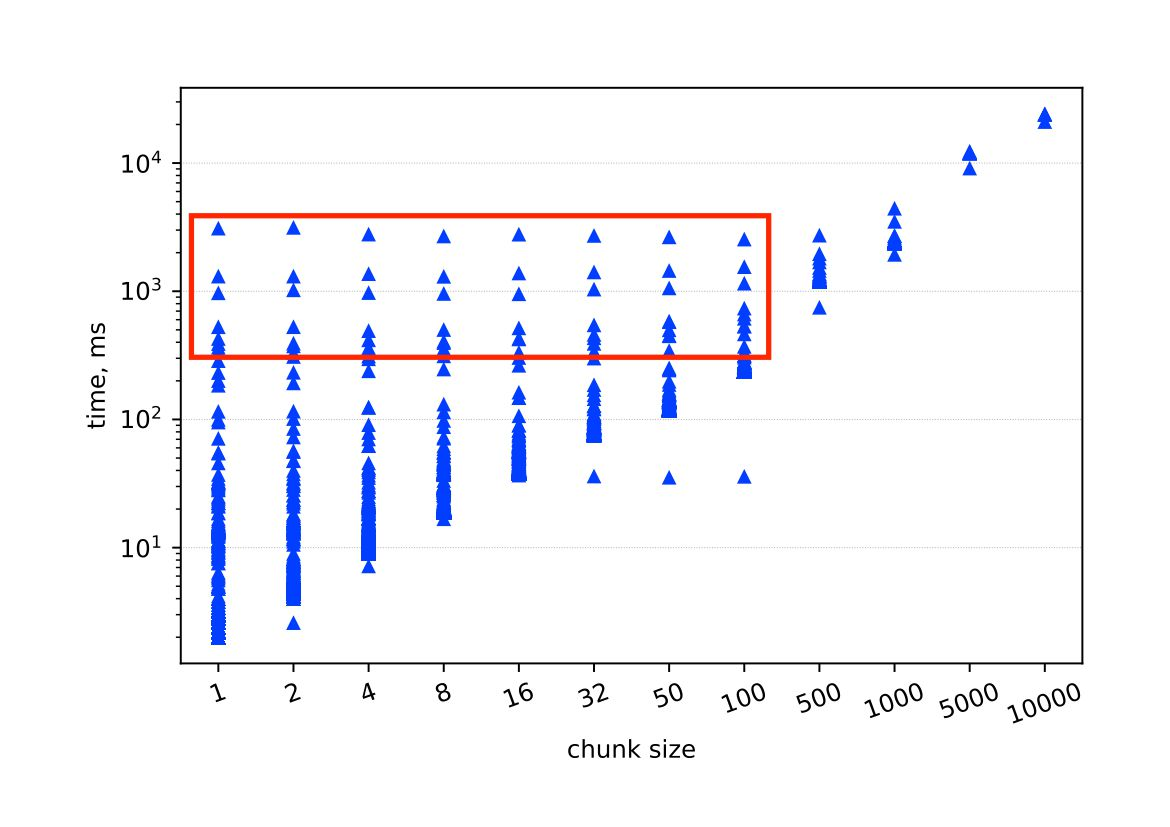
\includegraphics[width=\textwidth]{pics/st_old.pdf_1.jpg}  \caption{время выполнения \\ запросов}
    \label{1}
    \end{subfigure}%
    % \hfill
    \begin{subfigure}[b]{0.5\textwidth}
    \centering
    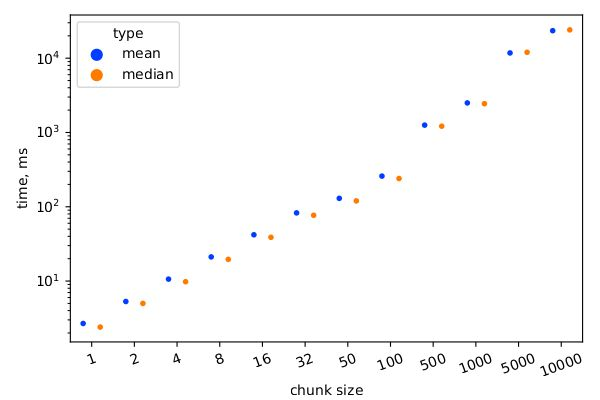
\includegraphics[width=\columnwidth]{pics/st_old_mean&median.pdf_1.jpg} \caption{медиана и среднее время выполнения запросов}
    \label{2}
    \end{subfigure} \caption{Грамматика $G_1$ на Enzyme}
    \label{old3}
    \begin{subfigure}[b]{0.5\textwidth}
    \centering
    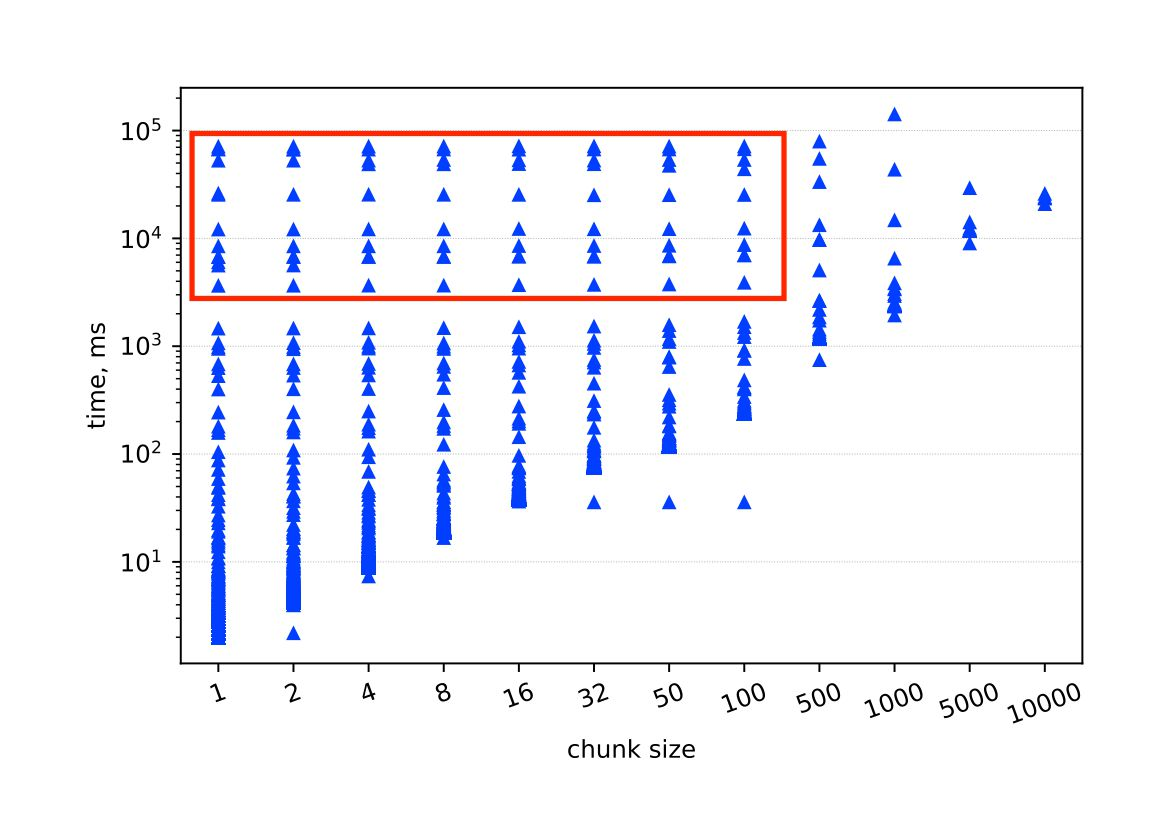
\includegraphics[width=\textwidth]{pics/subclass_old.pdf_1.jpg} \caption{время выполнения \\ запросов}
    \label{3}
    \end{subfigure}%
    % \hfill
    \begin{subfigure}[b]{0.5\textwidth}
    \centering
    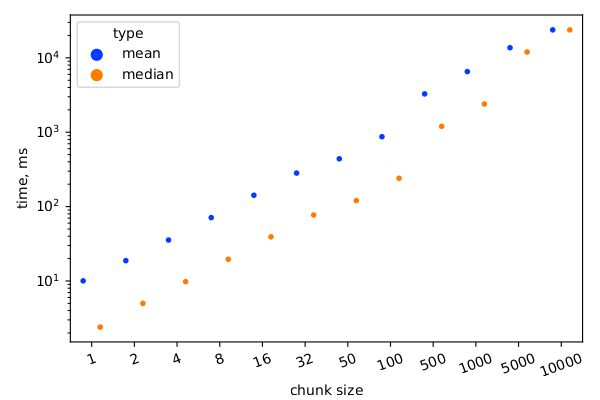
\includegraphics[width=\columnwidth]{pics/subclass_old_mean&median.pdf_1.jpg} \caption{медиана и среднее время выполнения запросов}
    \label{4}
    \end{subfigure} \caption{Грамматика $G_2$ на Enzyme}
    \label{old2}
        \end{figure}
    \begin{figure}[H]
        \begin{subfigure}[b]{0.5\textwidth}
    \centering
    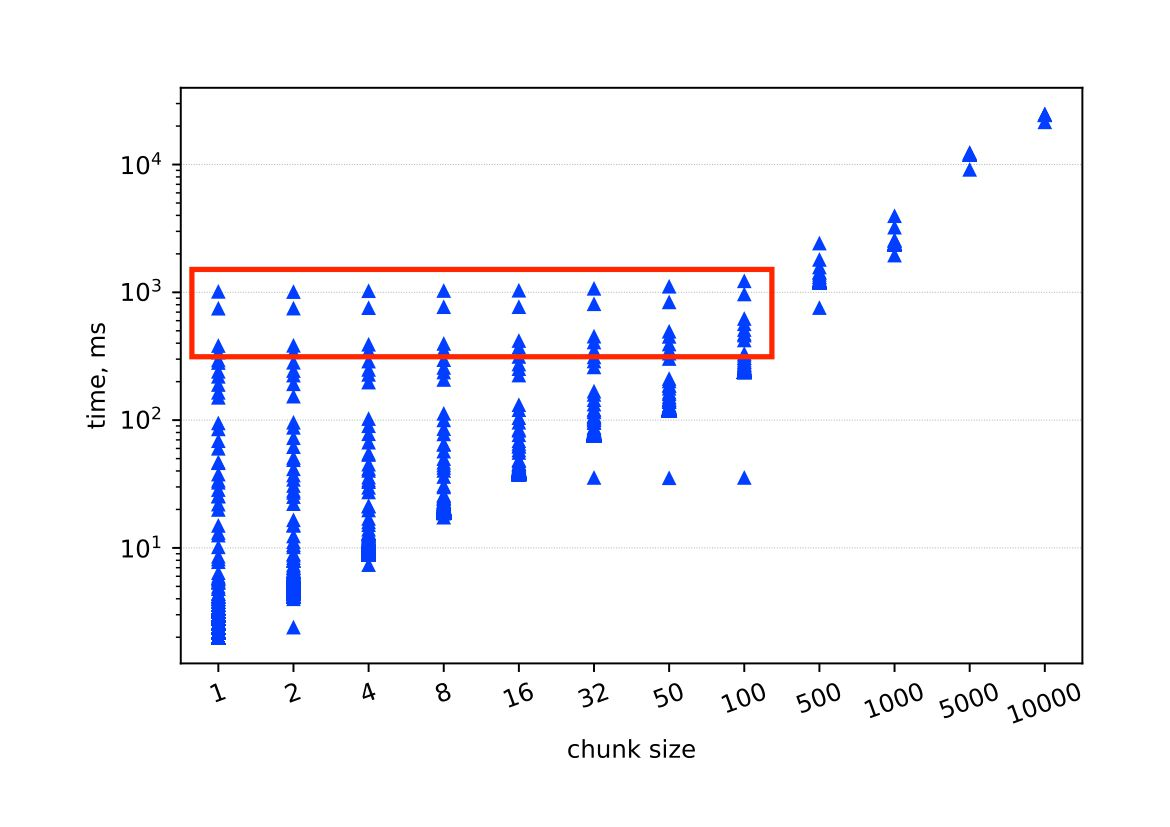
\includegraphics[width=\columnwidth]{pics/bt_old.pdf_1.jpg}  \caption{время выполнения \\ запросов}
    \label{5}
    \end{subfigure}%
    % \hfill
    \begin{subfigure}[b]{0.5\textwidth}
    \centering
    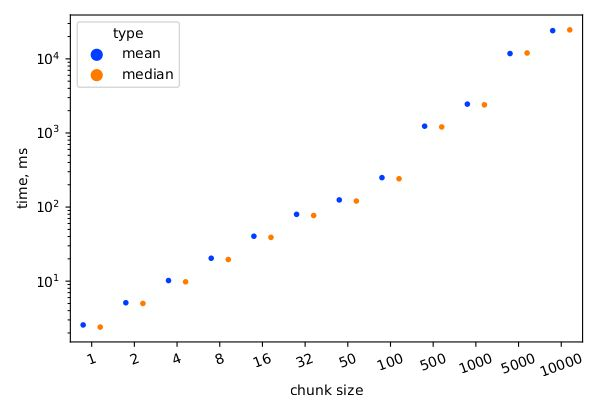
\includegraphics[width=\textwidth]{pics/bt_old_mean&median.pdf_1.jpg} \caption{медиана и среднее время выполнения запросов}
    \label{6}
    \end{subfigure} \caption{Грамматика $G_3$ на Enzyme}
\label{old}
\end{figure}

При анализе полученных данных были выделены следующие проблемы.
 \begin{itemize}
     \item Запросы от некоторых множеств вершин выполняются аномально долго по сравнению со скоростью выполнения других запросов того же типа. Для наглядности данные запросы выделены красным прямоугольником. Те же выводы подтверждаются разницей между значениями среднего арифметического и медианы.
     \item Enzyme является относительно небольшим графом, однако данные эксперименты явно показали, что уже на нем выполнение запросов от крупного множества вершин происходит критически медленно.
 \end{itemize} 
 
Несмотря на показанную в дипломной работе эффективность алгоритма при запросах от одной вершины до всех, данные проблемы в поведении ставят под вопрос его применимость на практике в том виде, в котором он есть.


\section{Оптимизация производительности\\ алгоритма}
В данном разделе описываются изменения, внесенные в реализацию алгоритма для повышения его производительности и устранения проблем, выявленных в разделе об экспериментальном исследовании существующего решения.

\subsection{Результаты профилирования существующего\\ решения}

Прежде чем приступить к оптимизациям кода было необходимо изучить распределение производительности алгоритма и выявить его <<узкие>> места. Самый удобный способ это сделать --- запуск алгоритмов с активным профилированием. В качестве инструмента для этого был выбран Java Flight Recorder (JFR), так как он интегрирован в виртуальную машину Java (JVM) и почти не вызывает накладных расходов на производительность. Анализ результатов запусков от <<плохих>> и от <<хороших>> множеств вершин производился на основе полученных flame-графиков. Flame-график --- диаграмма для трассировки стека, которая отражает процент времени от общего времени работы программы, затраченного в той или иной части кода. 

На основе анализа полученных результатов были сделаны выводы о том, что наибольшее количество процессорного времени тратится в основном методе класса Neo4jGraphInput --- nextSymbols. Данный метод используется для сопоставления текущего входа с терминалом грамматики. Он принимает идентификатор вершины и возвращает список меток (символов) на ребрах, выходящих из нее. При этом для получения данных меток неизбежно необходимо обратиться напрямую к базе Neo4j. Native Java API предоставляет удобный способ это сделать: получить итератор над множеством исходящих из вершины ребер с помощью метода getRelationships.iterator(). Однако, в результате анализа графика были сделаны выводы о том, что в текущей реализации практически всё процессорное время затрачивается на вычисления внутри базы. Полученные результаты профилирования послужили основанием для нижеописанного решения.

\subsection{Проблема производительности и предложенное решение}

В некоторых случаях алгоритм работал значительно медленнее по следующим причинам. Результатом вызова getRelationships.iterator() является итератор. Иными словами, возвращается не все данные в явном виде, а лишь объект, позволяющий перемещаться по содержимому контейнера. С другой стороны, результат со всеми выходящими метками сохраняется в виде списка в явном виде. Однако, заметим, что после сопоставления входа с терминалом, возможно, далеко не все метки понадобятся для дальнейшей работы алгоритма. Сохранение всех данных приводит к огромным накладным расходам (вплоть до переполнения кучи) в том случае, если степень вершины была очень большая, а большинство меток после соотнесения отбрасывается.
Таким образом, необходимо оптимизировать передачу меток из базы данных в дальнейшую обработку.

Довольно распространенным и обоснованным решением данной проблемы является использование Stream API. Stream в Java --- поток однотипных данных для однотипной обработки. Иначе говоря, он не является хранилищем данных, а является интерфейсом к источнику, откуда элементы берутся только по мере необходимости. Один из сценариев использования потоков в качестве возвращаемого типа метода выглядит следующим образом. В вызываемом методе надо задать обработку объектов с помощью одной или нескольких промежуточной операций, а в вызывающем --- конечную операцию. Метод nextSymbols был переписан в соответствии с данным сценарием для всех типов входных данных. Теперь источником данных является база данных Neo4j, промежуточной операцией --- фильтрация ребер по меткам, а конечной --- получение меток из возвращаемого методом nextSymbols потока. Таким образом, в данном методе была обеспечена потоковая обработка данных, извлекаемых посредством обращения к Neo4j.

Преобразованные алгоритмы были протестированы, а затем было запущено повторное профилирование. Его результаты подтвердили то, что внесенные изменения в способ получения меток из базы данных были верными и, тем самым, проблема медленной работы алгоритма при поиске ответа на ряд запросов была устранена. Более того, данные оптимизации в целом повлияли на скорость работы алгоритма в положительную сторону. 

Для того чтобы в этом убедиться, рассмотрим результаты замеров предложенной реализации в сравнении с изначальной реализацией алгоритма.
Ниже  на рис.\ref{old_new}-\ref{old_new3} отражены сравнительные графики временных замеров. Аналогично, дополнительно выделены медиана и среднее время ответа на запросы для каждого размера множества стартовых вершин. Приведенные результаты показывают, что улучшенная версия алгоритма при работе с реальными данными не только затрачивает на порядок меньше временных ресурсов, но также и в среднем более стабильна. Особенно хорошо это заметно графике медианы и среднего на рис.\ref{old_new2}, так как для измененного алгоритма эти два показателя практически сравнялись.

\begin{figure}[H]
    % \centering
    \begin{subfigure}[b]{0.5\textwidth}
    \centering
    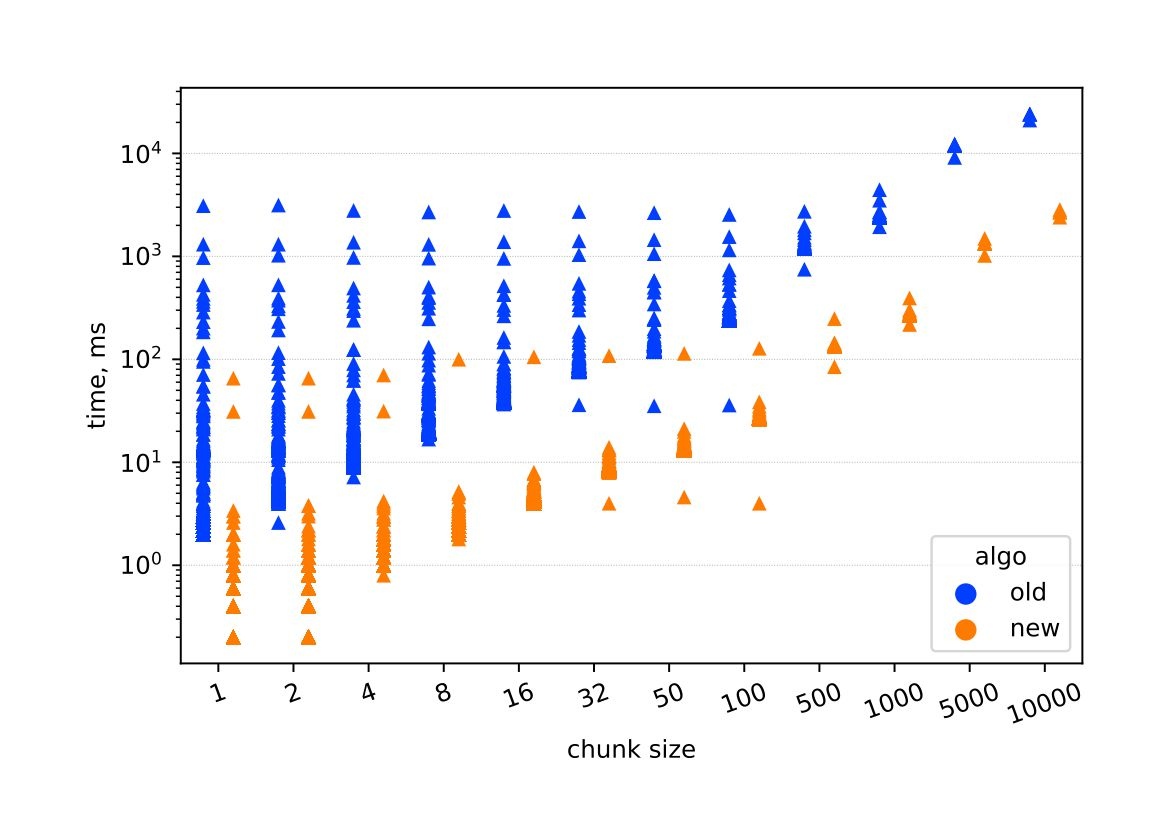
\includegraphics[width=\textwidth]{pics/st_old_new.pdf_1.jpg}  \caption{время выполнения \\ запросов}
    \label{fig:subim1}
    \end{subfigure}%
    % \hfill
    \begin{subfigure}[b]{0.5\textwidth}
    \centering
    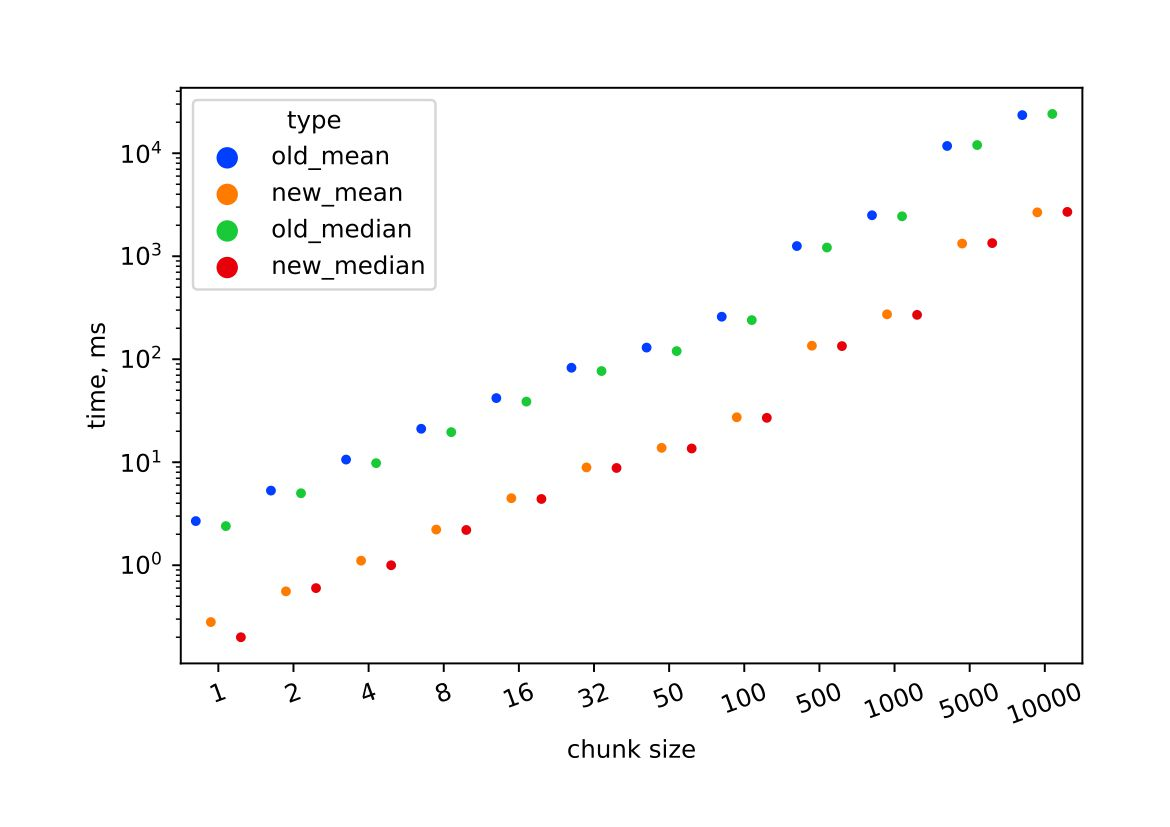
\includegraphics[width=\columnwidth]{pics/st_old_new_mean&median.pdf_1.jpg} \caption{медиана и среднее время выполнения запросов}
    \label{fig:subim2}
    \end{subfigure} \caption{Грамматика $G_1$ на Enzyme}
    \label{old_new}
        \end{figure} 
    \begin{figure}[H]
    \begin{subfigure}[b]{0.5\textwidth}
    \centering
    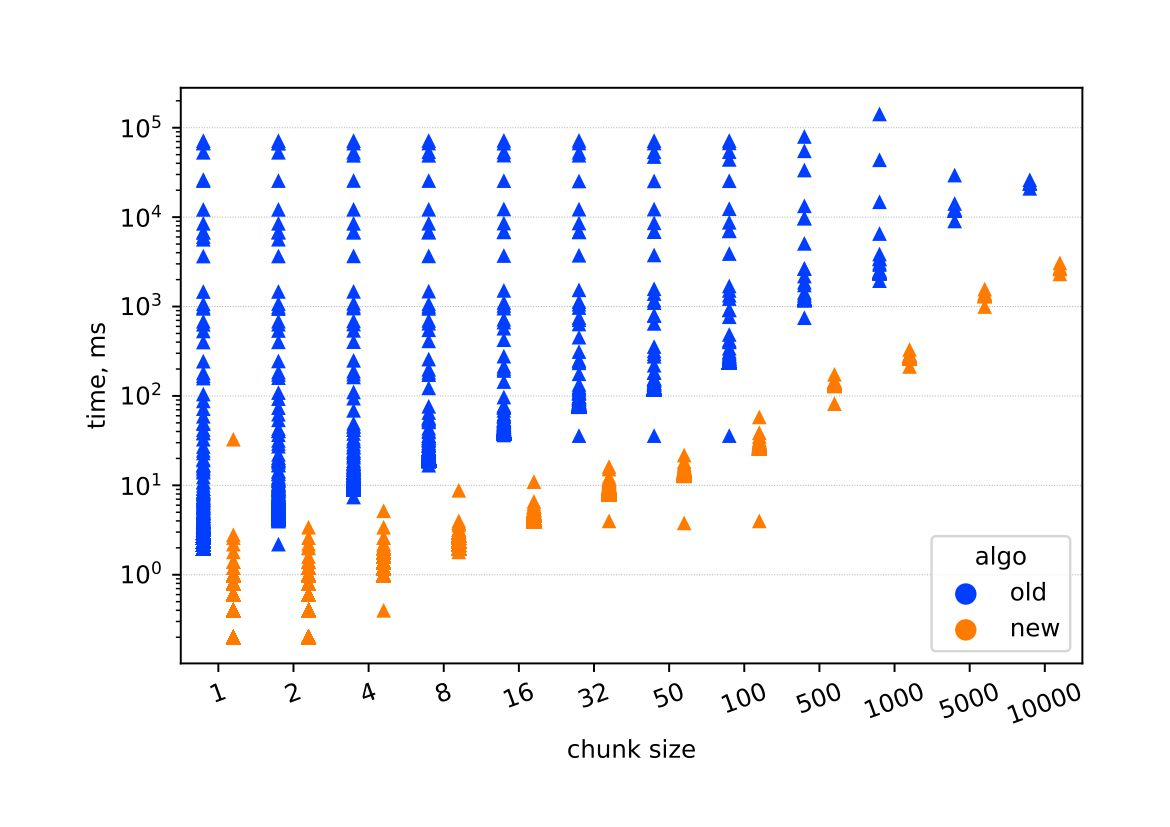
\includegraphics[width=\textwidth]{pics/subclass_old_new.pdf_1.jpg} \caption{время выполнения \\ запросов}
    \label{fig:subim1}
    \end{subfigure}%
    % \hfill
    \begin{subfigure}[b]{0.5\textwidth}
    \centering
    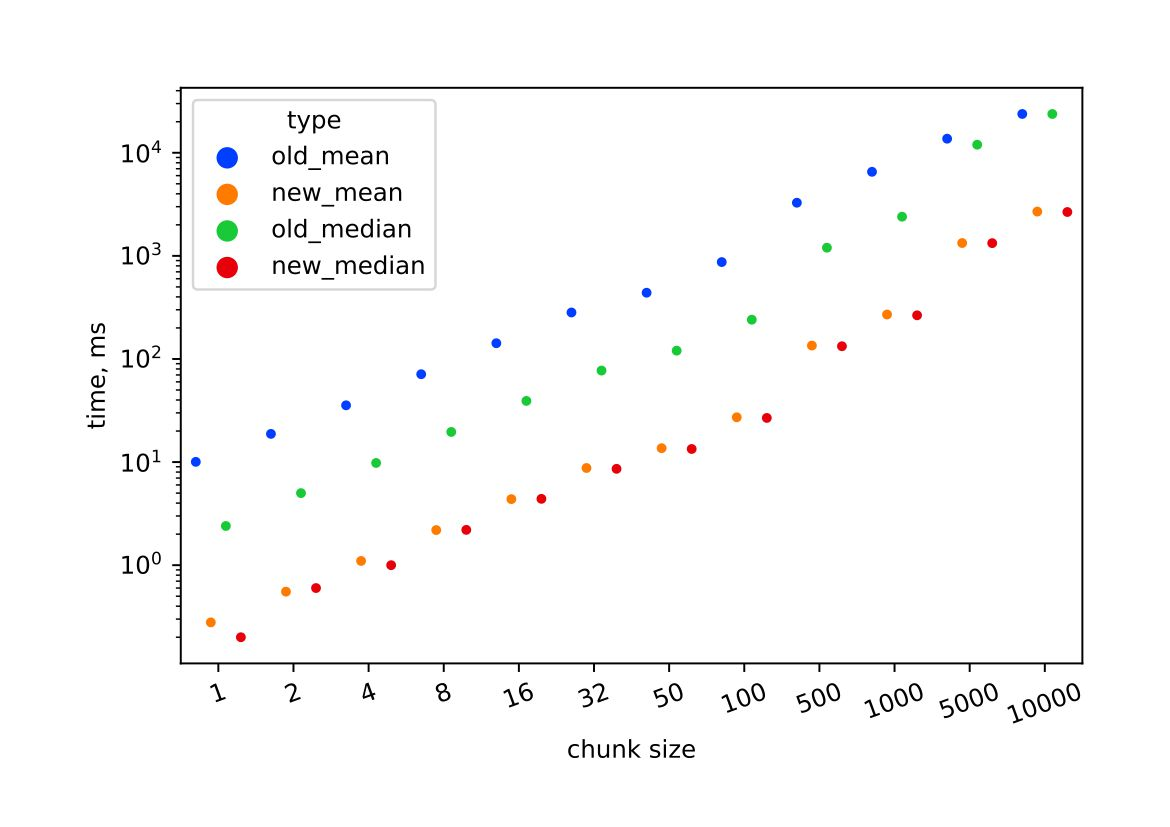
\includegraphics[width=\columnwidth]{pics/subclass_old_new_mean&median.pdf_1.jpg} \caption{медиана и среднее время выполнения запросов}
    \label{fig:subim2}
    \end{subfigure} \caption{Грамматика $G_2$ на Enzyme}
    \label{old_new2}
        \begin{subfigure}[b]{0.5\textwidth}
    \centering
    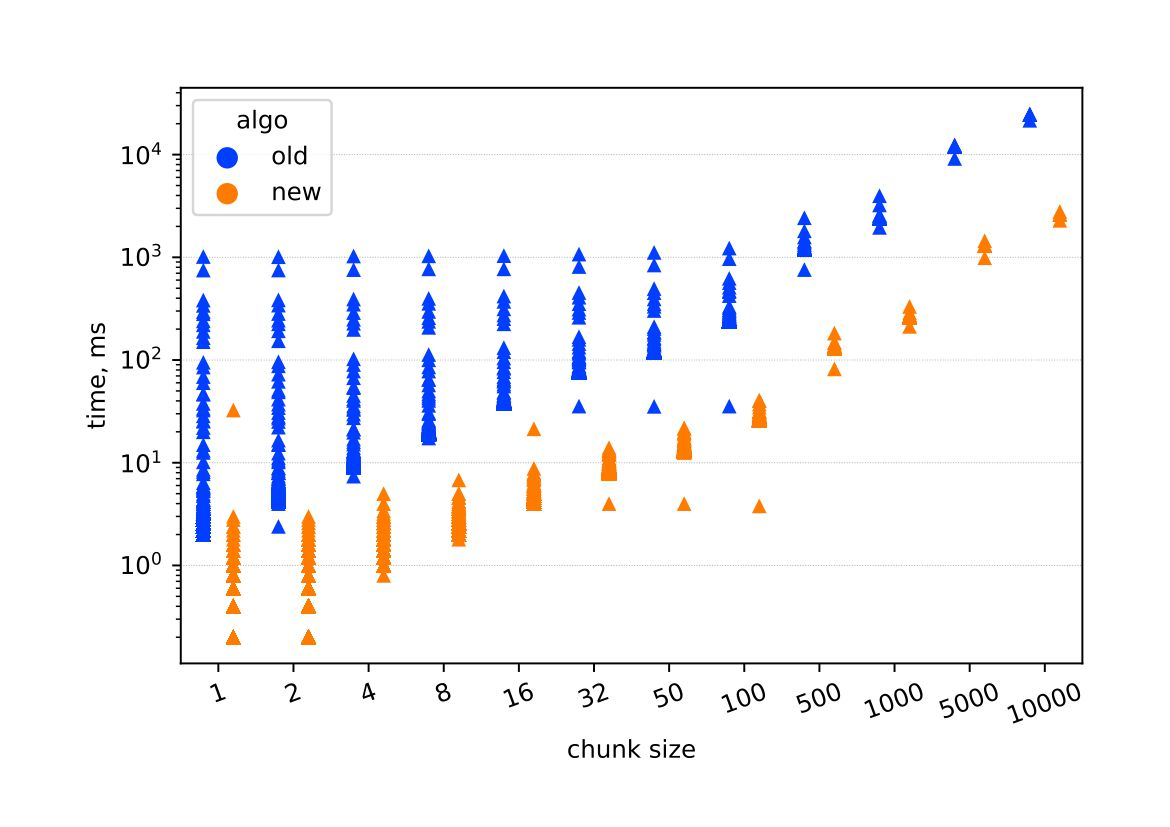
\includegraphics[width=\columnwidth]{pics/bt_old_new.pdf_1.jpg}  \caption{время выполнения \\ запросов}
    \label{fig:subim1}
    \end{subfigure}%
    % \hfill
    \begin{subfigure}[b]{0.5\textwidth}
    \centering
    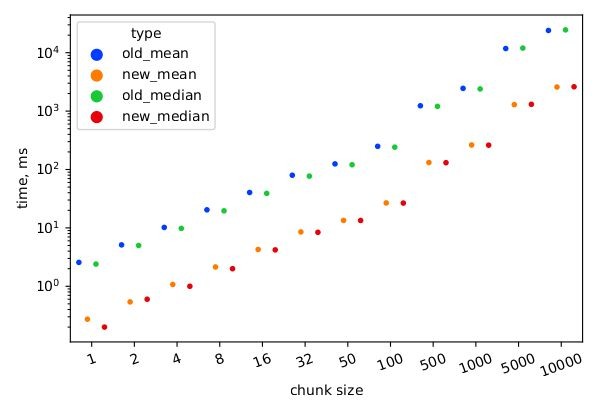
\includegraphics[width=\textwidth]{pics/bt_old_new_mean&median.pdf_1.jpg} \caption{медиана и среднее время выполнения запросов}
    \label{fig:subim2}
    \end{subfigure} \caption{Грамматика $G_3$ на Enzyme}
\label{old_new3}
\end{figure}

\section{Модификация алгоритма GLL}
В данном разделе описаны изменения, которые были внесены в работу алгоритма для решения задачи достижимости с ограничениями, заданными в виде контекстно-свободных грамматик.

На рис.\ref{fig:sppf} представлена диаграмма основных классов Iguana после того, как алгоритм был модифицирован и добавлена поддержка получения в качестве результата лишь пар достижимостей. Зеленым цветом на этой диаграмме отмечены классы и методы, которые на данном этапе работы были изменены.
\begin{figure}[H]
\centering
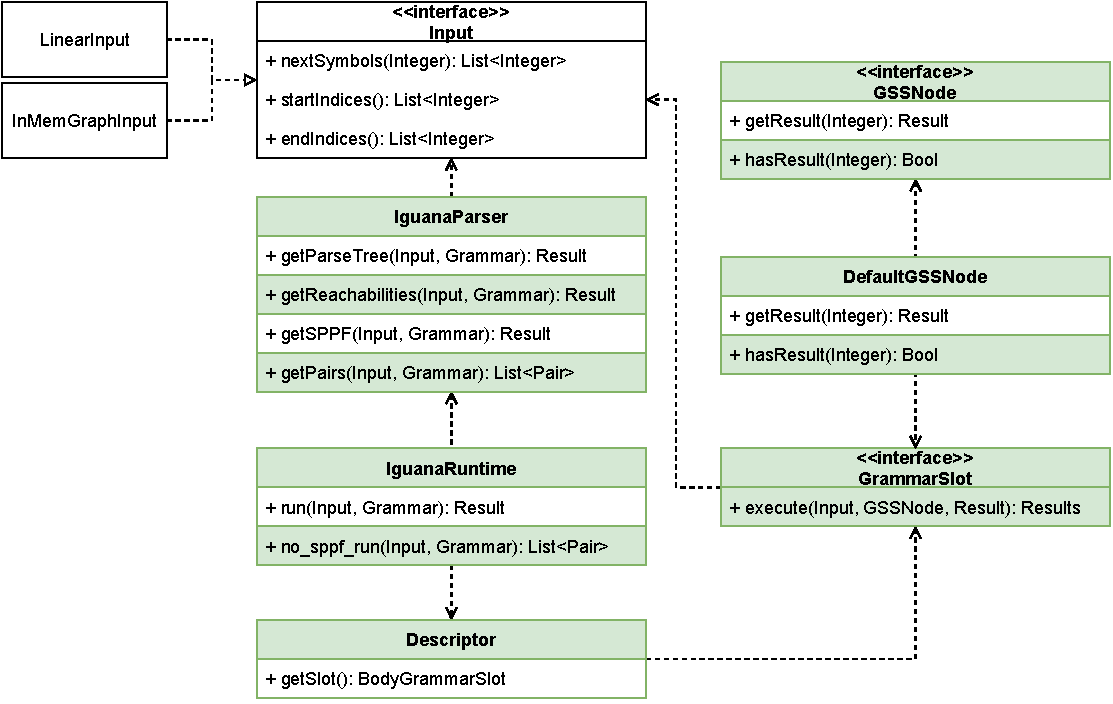
\includegraphics[width=\textwidth]{pics/sppf.pdf}
\caption{Диаграмма классов Iguana после модификаций для поддержки опции отключения SPPF}
\label{fig:sppf}
\end{figure}

Результатом работы алгоритма GLL на графе является компактное представление леса разбора.
Посредством обхода данного дерева можно восстановить пути, удовлетворяющие запросу.

В ходе работы алгоритма при обработке вершины стека GSS создавался текущий узел SPPF, иначе говоря, фрагмент дерева, которое построено на момент создания новой вершины стека. Данная информация сохранялась на ребрах GSS, после чего полученный дескриптор добавлялся в очередь дескрипторов.
В случае решения задачи достижимости необходимость в поддержании SPPF отпадает, так как в качестве результата достаточно возвращать пары начальных и конечных вершин, а сами пути восстанавливать не надо. Поведение алгоритма было модифицировано в описанном выше сценарии соответствующим образом. Создание SPPF вершин и добавление их в дескрипторы предотвращено, а для всех зависимых методов была добавлена новая сигнатура.
Таким образом,  была расширена функциональность решения и добавлена возможность запуска алгоритма без мемоизации SPPF.

\section{Экспериментальное исследование разработанного решения}
    
Полученное решение было протестировано на том же оборудовании. Так как после проведения оптимизаций объем потребляемых процессорных ресурсов значительно уменьшился для обоих алгоритмов, для проведения экспериментального исследования появилась возможность включить в набор данных граф Geospecies.

На рис.\ref{enz1}-\ref{sss} приведены результаты замеров производительности для графа Enzyme, а также для каждого запроса соответственно приведены графики зависимостей количества достижимых вершин от стартового множества и графики медиан и среднего времени выполнения запросов.
На рис.\ref{geo}-\ref{ssss} приведены аналогичные результаты для Geospecies.

На всех графиках четко прослеживается, что чем крупнее выбранное множество стартовых вершин, тем заметнее становится разница в скорости работы алгоритмов. Время работы алгоритма, который строит SPPF, прямо пропорционально размеру ответа на запрос, так как чем больше путей попадает в ответ, тем больше количество процессорных ресурсов уходит на их мемоизацию. С другой стороны, время работы алгоритма, который не стоит SPPF, практически не увеличивается по мере роста количества возвращаемых пар вершин, что означает, что он может быть применен для решения задачи достижимости на реальных графах.

Анализ полученных результатов показал, что модифицированный алгоритм GLL без построения SPPF может быть эффективно применен для решения задачи поиска достижимостей в графе с контекстно-свободными ограничениями на реальных данных.
Полученные результаты делают актуальными дальнейшие исследования, направленные как на улучшение данного алгоритма и реализации, так и на полноценную интеграцию его в графовую базу данных Neo4j.

\begin{figure}[H]
    \begin{center}
    % \hfill
    \begin{subfigure}[b]{0.8\textwidth}
    \centering
    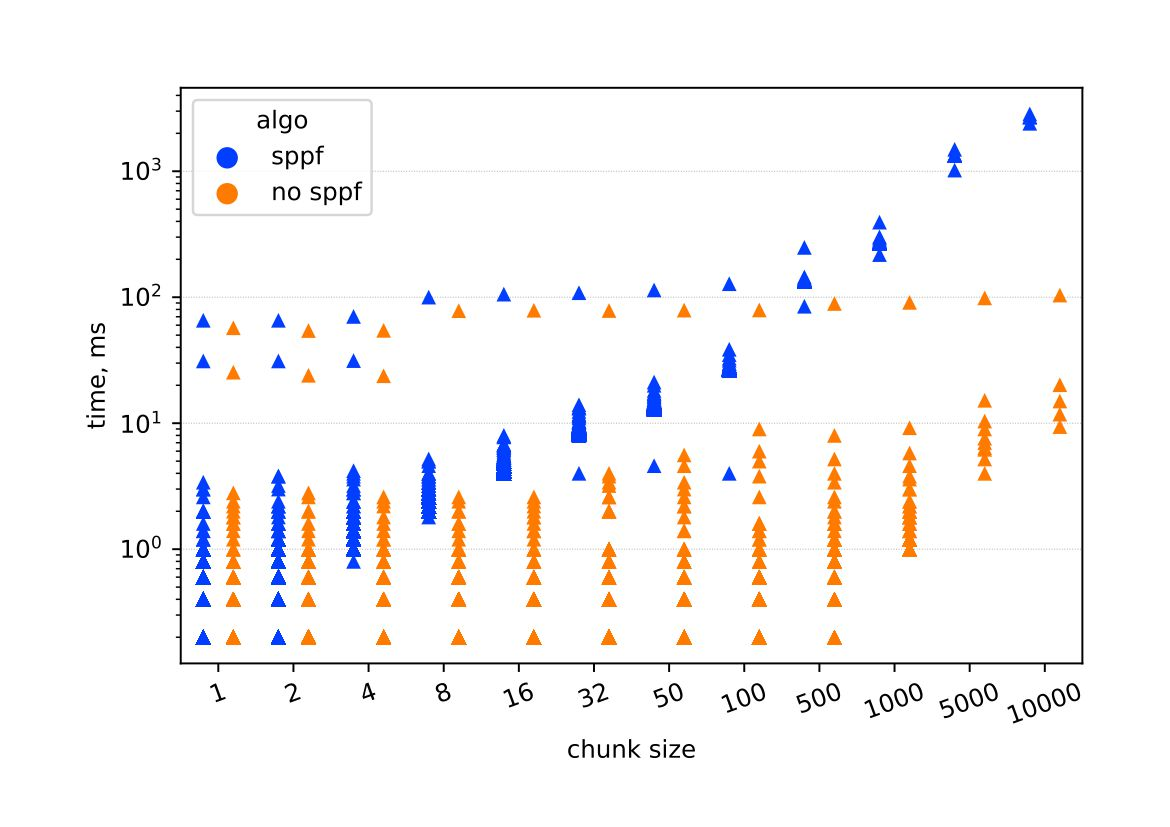
\includegraphics[width=\textwidth]{pics/enzyme_sppf_st.pdf_1.jpg}  \caption{время выполнения запросов}
    \label{fig:subim1}
    \end{subfigure}%
    \end{center}
    \begin{subfigure}[b]{0.5\textwidth}
    \centering
    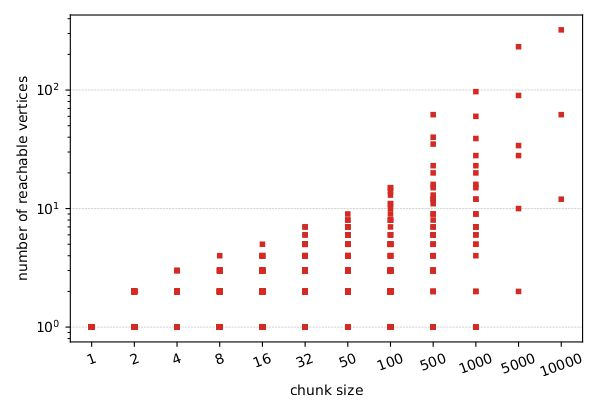
\includegraphics[width=\columnwidth]{pics/enzyme_ans_st.pdf_1.jpg} \caption{размер ответов на запросы}
    \label{fig:subim2}
    \end{subfigure} 
        \hfil
    \begin{subfigure}[b]{0.5\textwidth}
    \centering
    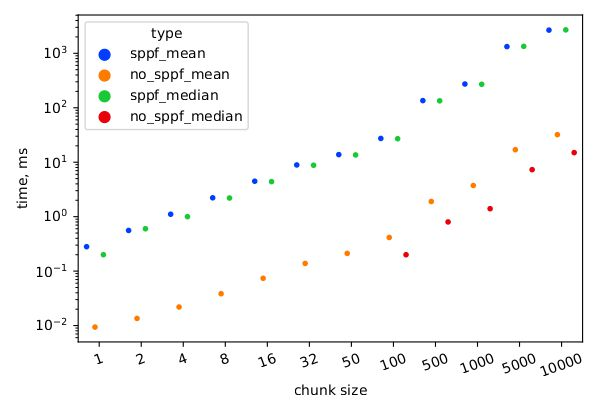
\includegraphics[width=\textwidth]{pics/st_sppf_mean&median.pdf_1.jpg}  \caption{медиана и среднее время на запросы}
    \label{fig:subim0}
    \end{subfigure} \caption{Грамматика $G_1$ на Enzyme}
    \label{enz1}
    \end{figure}
    \begin{figure}[H]
    \begin{center}
    \begin{subfigure}[b]{0.8\textwidth}
    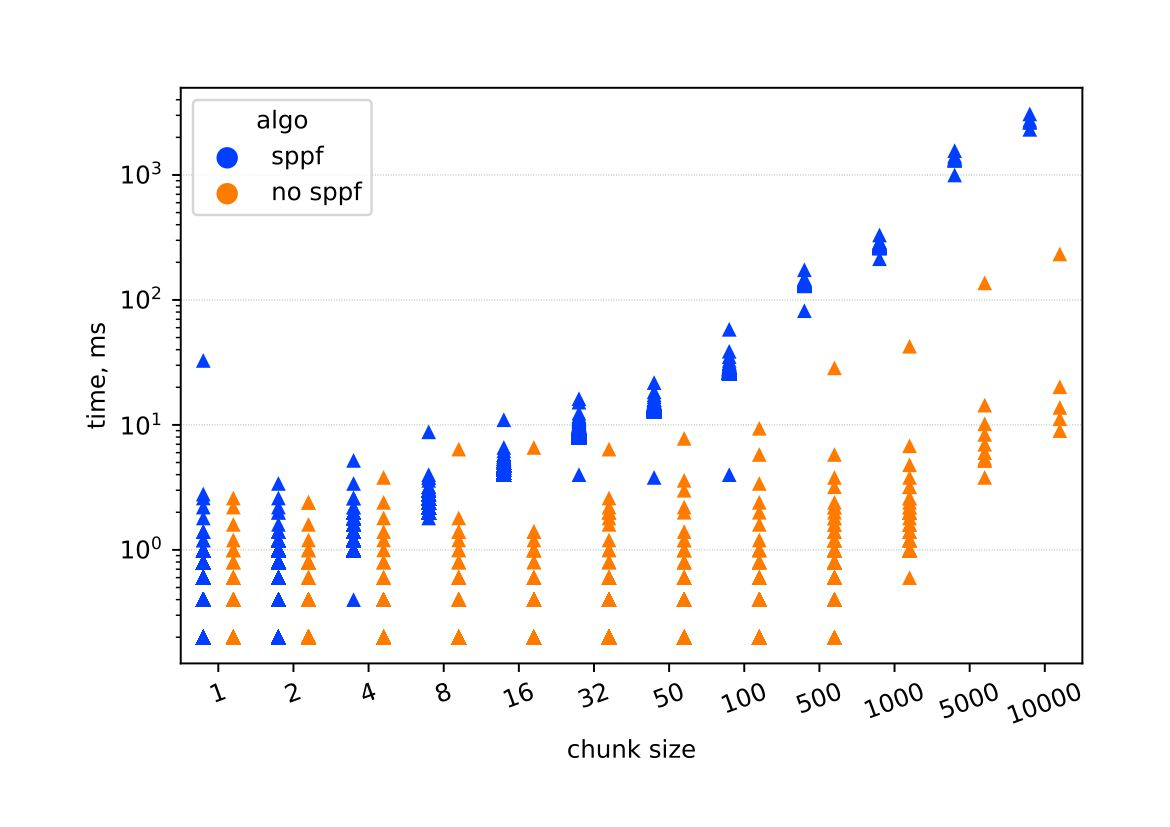
\includegraphics[width=\textwidth]{pics/enzyme_sppf_subclass.pdf_1.jpg} \caption{время выполнения запросов}
    \label{fig:subim1}
    \end{subfigure}%
    \end{center}
    \begin{subfigure}[b]{0.5\textwidth}
    \centering
    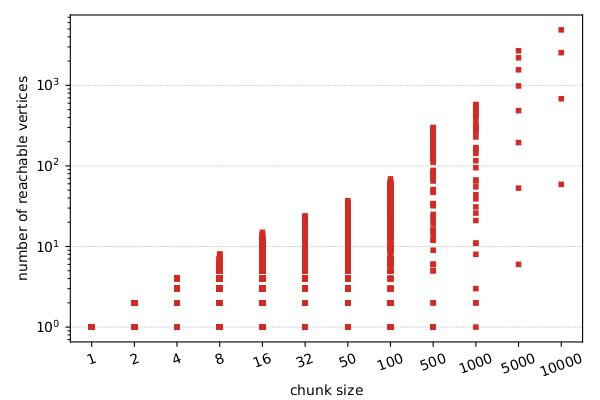
\includegraphics[width=\columnwidth]{pics/enzyme_subclass_ans_st.pdf_1.jpg} \caption{размер ответов на запросы}
    \label{fig:subim2}
    \end{subfigure}
    \begin{subfigure}[b]{0.5\textwidth}
    \centering
    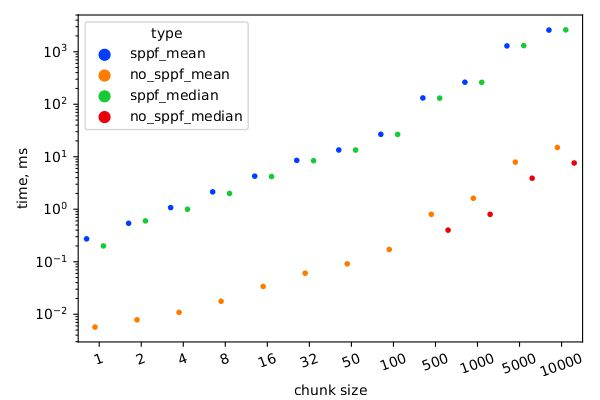
\includegraphics[width=\textwidth]{pics/subclass_sppf_mean&median.pdf_1.jpg}  \caption{медиана и среднее время на запросы}
    \label{fig:subim0}
    \end{subfigure} \caption{Грамматика $G_2$ на Enzyme}
        \end{figure}
    \begin{figure}[H]
    \begin{center}
        \begin{subfigure}[b]{0.8\textwidth}
    \centering
    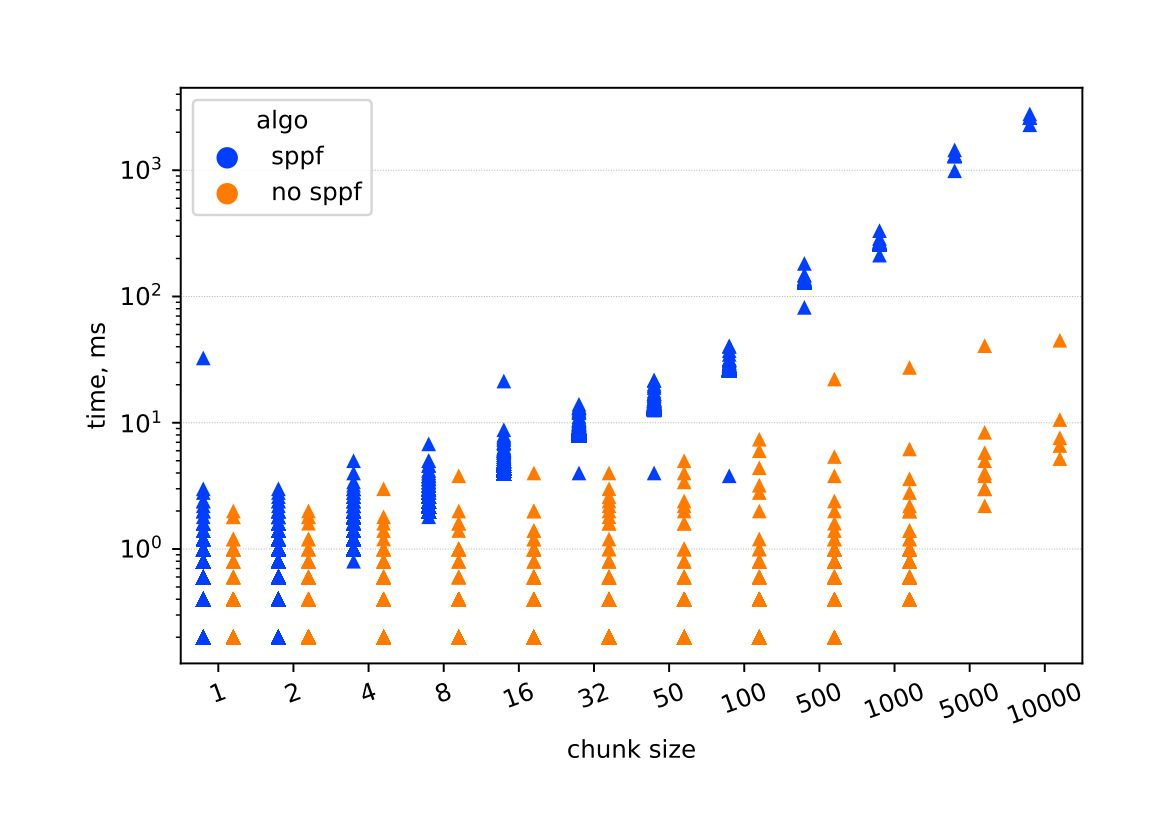
\includegraphics[width=\columnwidth]{pics/enzyme_sppf_bt.pdf_1.jpg}  \caption{время выполнения запросов}
    \label{fig:subim1}
    \end{subfigure}%
    \end{center}
    \begin{subfigure}[b]{0.5\textwidth}
    \centering
    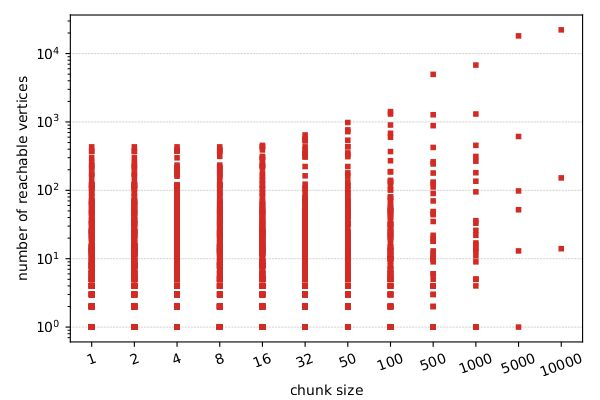
\includegraphics[width=\textwidth]{pics/enzyme_ans_bt.pdf_1.jpg} \caption{размер ответов на запросы}
    \label{fig:subim2}
    \end{subfigure}
        \begin{subfigure}[b]{0.5\textwidth}
    \centering
    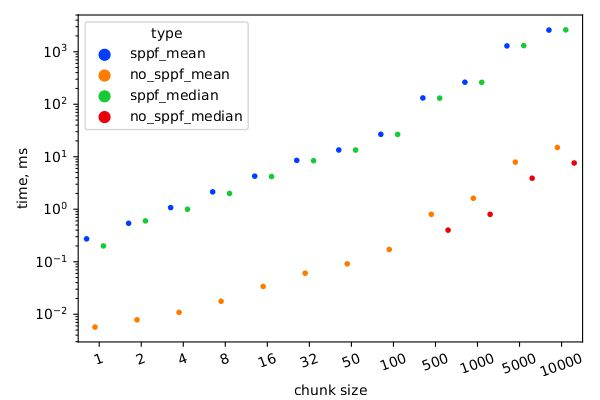
\includegraphics[width=\textwidth]{pics/bt_sppf_mean&median.pdf_1.jpg}  \caption{медиана и среднее время на запросы}
    \label{fig:subim0}
    \end{subfigure} \caption{Грамматика $G_3$ на Enzyme}
\label{sss}
\end{figure}

\begin{figure}[H]
    \begin{center}
    \begin{subfigure}[b]{0.8\textwidth}
    \centering
    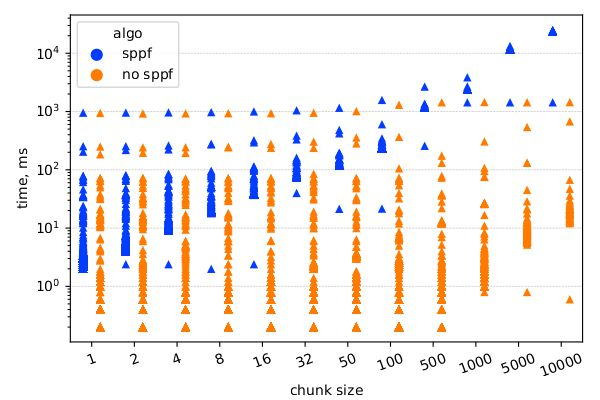
\includegraphics[width=\textwidth]{pics/geospecies_sppf_st.pdf_1.jpg} \caption{время выполнения запросов}
    \label{fig:subim1}
    \end{subfigure}%
    \end{center}
    \begin{subfigure}[b]{0.5\textwidth}
    \centering
    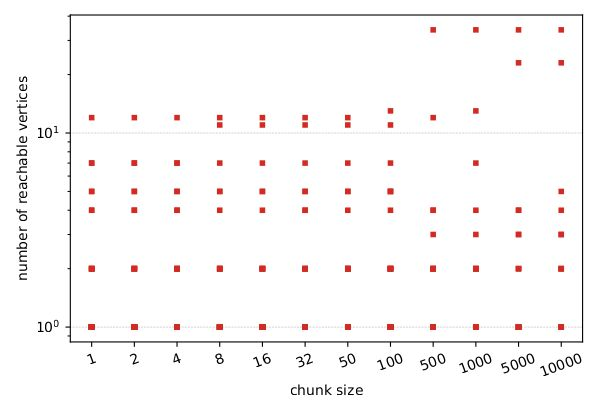
\includegraphics[width=\textwidth]{pics/geospecies_ans_st.pdf_1.jpg} \caption{размер ответов на запросы}
    \label{fig:subim2}
    \end{subfigure}         \begin{subfigure}[b]{0.5\textwidth}
    \centering
    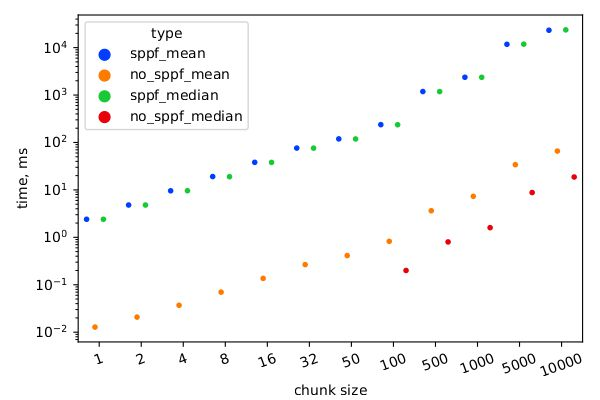
\includegraphics[width=\textwidth]{pics/geo_st_mean&median.pdf_1.jpg}  \caption{медиана и среднее время на запросы}
    \label{fig:subim0}
    \end{subfigure} \caption{Грамматика $G_1$ на Geospecies}
    \label{geo}
    \end{figure}
    \begin{figure}[H]
    \begin{center}
    \begin{subfigure}[b]{0.8\textwidth}
    \centering
    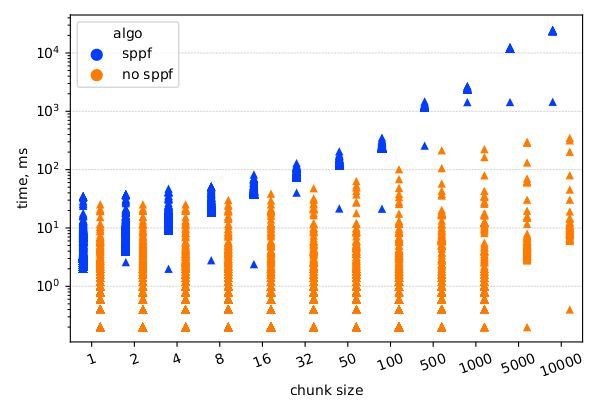
\includegraphics[width=\textwidth]{pics/geospecies_sppf_bt.pdf_1.jpg} \caption{время выполнения запросов}
    \label{fig:subim3}
    \end{subfigure}%
    \end{center}
    \begin{subfigure}[b]{0.5\textwidth}
    \centering
    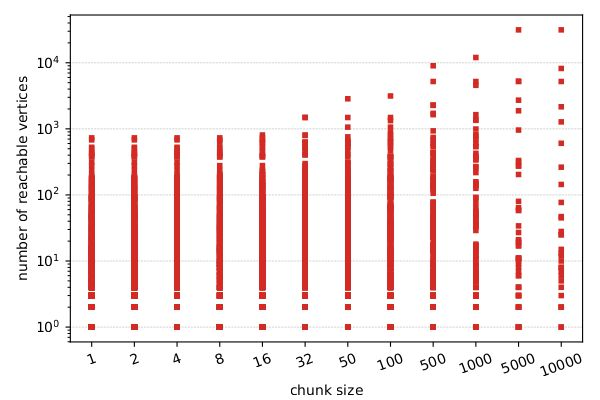
\includegraphics[width=\textwidth]{pics/geospecies_ans_bt.pdf_1.jpg} \caption{размер ответов на запросы}
    \label{fig:subim4} 
    \end{subfigure}
        \begin{subfigure}[b]{0.5\textwidth}
    \centering
    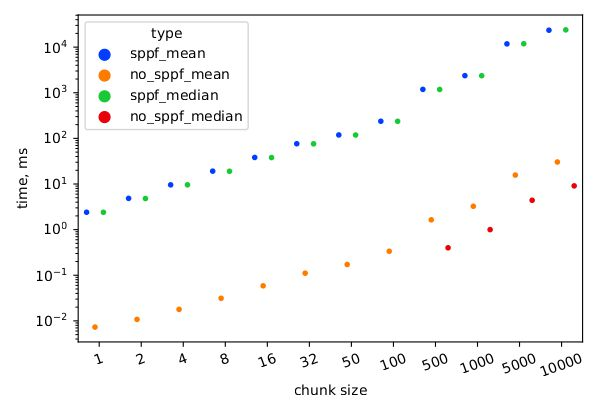
\includegraphics[width=\textwidth]{pics/geo_bt_mean&median.pdf_1.jpg}  \caption{медиана и среднее время на запросы}
    \label{fig:subim0}
    \end{subfigure} \caption{Грамматика $G_3$ на Geospecies}

\label{ssss}
\end{figure}

\section{Заключение}

В рамках производственной практики были выполнены следующие задачи.
\begin{itemize}
    \item Проведен анализ кода и его рефакторинг.
    \item Выявлены и устранены проблем производительности текущей реализации GLL алгоритма.
    \item Добавлена возможность отключения построения SPPF и возврата информации лишь о достижимостях в графе.
    \item Проведено экспериментальное исследование на реальных данных и сравнение полученного решения с уже существующим.
\end{itemize}

Дальнейшими направлениями для развития работы являются:
\begin{itemize}
    \item сравнение полученного решения для Neo4j с другими графовыми базами данных на регулярных запросах;
    \item сравнение полученного решения для Neo4j с другими графовыми базами данных и самостоятельными инструментами на кон-текстно-свободных запросах в рамках задачи статического анализа кода;
    \item публикация алгоритма и результатов экспериментального исследования.
\end{itemize}
\setmonofont[Mapping=tex-text]{CMU Typewriter Text}
\bibliographystyle{ugost2008ls}
\bibliography{coursework.bib}
\end{document}